\documentclass[conference]{IEEEtran}
\IEEEoverridecommandlockouts
\usepackage{cite}
\usepackage{amsmath,amssymb,amsfonts}
\usepackage{graphicx}
\usepackage{textcomp}
\usepackage{xcolor}
\usepackage{booktabs}
\usepackage{tikz}
\usetikzlibrary{arrows.meta,positioning}
\def\BibTeX{{\rm B\kern-.05em{\sc i\kern-.025em b}\kern-.08em
    T\kern-.1em\lower.7ex\hbox{E}\kern-.125em X}}

\begin{document}

\title{Real-Time American Sign Language Alphabet Recognition Using MediaPipe Hand Localization and a Fine-Tuned EfficientNet-B0}

\author{
\IEEEauthorblockN{Author One}
\IEEEauthorblockA{\textit{Department of Computer Science} \\
\textit{Institution Name}\\
City, Country \\
email@example.com}
\and
\IEEEauthorblockN{Author Two}
\IEEEauthorblockA{\textit{Department of Computer Science} \\
\textit{Institution Name}\\
City, Country \\
email@example.com}
\and
\IEEEauthorblockN{Author Three}
\IEEEauthorblockA{\textit{Department of Computer Science} \\
\textit{Institution Name}\\
City, Country \\
email@example.com}
\and
\IEEEauthorblockN{Author Four}
\IEEEauthorblockA{\textit{Department of Computer Science} \\
\textit{Institution Name}\\
City, Country \\
email@example.com}
\and
\IEEEauthorblockN{Author Five}
\IEEEauthorblockA{\textit{Department of Computer Science} \\
\textit{Institution Name}\\
City, Country \\
email@example.com}
}

\maketitle

\begin{abstract}
Fingerspelling lets deaf and hard-of-hearing signers spell names and technical terms that have no dedicated sign, yet most hearing people cannot read it. We present a lightweight, real-time system that recognizes the 26 static letters of the American Sign Language (ASL) alphabet from a single RGB camera. The system localizes the signing hand with MediaPipe, crops a square region around the detected landmarks, and classifies the crop with an ImageNet-pretrained EfficientNet-B0 fine-tuned end to end. We compare three training configurations on a stratified 80/10/10 split of a public 10{,}873-image dataset: full images, hand crops, and hand crops with a robust augmentation policy (50\% horizontal flips, stronger photometric changes, blur and grayscale). All three models, each with only 4.04\,M parameters, exceed 98.9\% accuracy on the 1{,}088-image held-out test split (98.90\%, 99.36\% and 99.45\%). Remaining errors concentrate on a few handshapes that differ mainly in thumb placement and on the motion-based letters J and Z. The classifier runs in about 13\,ms per image on a laptop GPU, enabling a live webcam demonstration. The evaluation is in-distribution only: generalization to unseen signers and capture conditions is not assessed and is left to future work.
\end{abstract}

\begin{IEEEkeywords}
sign language recognition, ASL fingerspelling, EfficientNet, MediaPipe, transfer learning, data augmentation
\end{IEEEkeywords}

\section{Introduction}
Sign languages are the primary means of communication for millions of deaf and hard-of-hearing people worldwide. Most hearing people never learn them, which creates a persistent communication barrier in education, healthcare and public services. Automatic sign language recognition (SLR) aims to reduce this barrier, and it has attracted sustained research interest, as documented by several surveys~\cite{rastgoo2021survey,cheok2019review,koller2020quantitative}.

Within American Sign Language (ASL), \emph{fingerspelling} represents each letter of the English alphabet with a distinct handshape. It is used for proper nouns, technical vocabulary and words without an established sign, and it forms a significant fraction of everyday signing~\cite{shi2018fingerspelling}. Of the 26 letters, 24 are \emph{static} handshapes, whereas J and Z are defined by a hand \emph{movement}. Static fingerspelling is therefore a natural and well-defined first target for image-based recognition: it is a fine-grained 26-class problem in which the discriminative information is concentrated in the shape of the fingers and thumb.

Early fingerspelling recognizers relied on hand-crafted features and depth sensors~\cite{pugeault2011spelling,kang2015realtime}, and convolutional neural networks (CNNs) later became the dominant approach~\cite{pigou2014sign}. Modern pretrained CNNs make it possible to obtain very high accuracy on benchmark data with modest compute through transfer learning~\cite{yosinski2014transferable,pan2010survey}. However, benchmark accuracy on a random split of a single dataset can be misleading: images from the same dataset share signers, cameras and backgrounds, so the test split is not independent of the training distribution in the sense that matters for deployment~\cite{torralba2011unbiased}. A system intended for a live webcam must cope with different hands, lighting and backgrounds.

This paper builds and evaluates such a system, and is explicit about what its evaluation does and does not show. Our contributions are as follows.
\begin{enumerate}
\item We build a complete, real-time recognition pipeline that combines MediaPipe hand localization~\cite{zhang2020mediapipe} with a fine-tuned EfficientNet-B0~\cite{tan2019efficientnet} classifier, small enough (4.04\,M parameters) to run live on a laptop GPU.
\item We compare three input and augmentation configurations (full image, hand crop, hand crop with robust augmentation) under an identical, seeded, stratified split.
\item We report held-out accuracy, macro-F1, per-class metrics and a confusion matrix for each configuration under an identical, seeded, stratified split, and we state explicitly that these are in-distribution measurements.
\item We analyze the remaining errors, which concentrate on visually similar handshapes and on the motion-based letters J and Z.
\end{enumerate}

The remainder of the paper is organized as follows. Section~\ref{sec:related} reviews related work. Section~\ref{sec:method} describes the dataset, pipeline and training. Section~\ref{sec:setup} gives the experimental setup. Section~\ref{sec:results} presents results, Section~\ref{sec:discussion} discusses them and their limitations, and Section~\ref{sec:conclusion} concludes.

\section{Related Work}
\label{sec:related}
\subsection{Sign Language and Fingerspelling Recognition}
Surveys of SLR describe a progression from glove- and sensor-based systems to vision-based approaches and, more recently, to deep models that learn features directly from pixels~\cite{cheok2019review,rastgoo2021survey}. Koller~\cite{koller2020quantitative} compares the state of the art quantitatively and highlights that results obtained on small, controlled datasets often do not transfer to realistic conditions. For fingerspelling in particular, Pugeault and Bowden~\cite{pugeault2011spelling} used Gabor-filter features from color and depth data for real-time ASL alphabet recognition with a Kinect sensor. Kang et al.~\cite{kang2015realtime} applied a CNN to depth maps, and Pigou et al.~\cite{pigou2014sign} used CNNs for recognizing gestures from video. Shi et al.~\cite{shi2018fingerspelling} moved to ``in the wild'' fingerspelling, demonstrating that unconstrained videos are substantially harder than studio recordings. At the word level, Li et al.~\cite{li2020word} released a large-scale video dataset and compared recognition methods, illustrating the scale needed for open-vocabulary SLR.

\subsection{Efficient CNN Architectures and Transfer Learning}
The success of deep learning in vision followed large-scale training on ImageNet~\cite{deng2009imagenet,krizhevsky2012imagenet}. Deeper architectures such as VGG~\cite{simonyan2015very} and residual networks~\cite{he2016deep} improved accuracy, while efficiency-oriented designs such as MobileNets~\cite{howard2017mobilenets,sandler2018mobilenetv2} target mobile and embedded deployment. EfficientNet~\cite{tan2019efficientnet} scales depth, width and resolution jointly with a compound coefficient and achieves strong accuracy per parameter. Vision transformers~\cite{dosovitskiy2021image} are an alternative family that typically requires more data or pretraining. Features learned on ImageNet transfer well to new tasks, particularly in the lower layers~\cite{yosinski2014transferable}, which makes fine-tuning a pretrained network the standard strategy when the target dataset is comparatively small~\cite{pan2010survey}.

\subsection{Hand Localization}
Reliable hand localization removes background clutter before classification. MediaPipe provides a cross-platform framework for building perception pipelines~\cite{lugaresi2019mediapipe}, and its hand tracking solution predicts 21 three-dimensional hand landmarks from a single RGB frame in real time on mobile hardware~\cite{zhang2020mediapipe}. We use the landmark extent to define a tight, square crop around the hand.

\subsection{Augmentation and Dataset Shift}
Data augmentation is a principal tool for improving generalization~\cite{shorten2019survey}. Dataset shift, in which training and deployment distributions differ, is a well-studied cause of performance degradation~\cite{quinonero2009dataset}, and the theory of learning from different domains formalizes why error on a source domain may not bound error on a target domain~\cite{bendavid2010theory}. Torralba and Efros~\cite{torralba2011unbiased} showed that even large vision datasets carry strong, identifiable biases. These observations motivate our explicit statement that our evaluation is in-distribution.

\section{Method}
\label{sec:method}

\subsection{Dataset}
We use a publicly available ASL alphabet image dataset containing 10{,}873 labeled images of the 26 letters (between 380 and 420 images per class; the test split contains 38 to 42 images per class). The images vary in resolution, background and hand appearance; many are clean, close-up photographs on plain backgrounds, and some are webcam-style frames. We create a single stratified split with a fixed random seed (42): 80\% training (8{,}698 images), 10\% validation (1{,}087) and 10\% test (1{,}088). The same split indices are used for every model, so differences between models cannot be attributed to different data. The validation split is used only to select the best epoch; the test split is used once per model for final reporting.

\subsection{Pipeline Overview}
Fig.~\ref{fig:pipeline} shows the pipeline. A frame is passed to the MediaPipe hand landmarker, which returns 21 landmarks for the first detected hand. The axis-aligned bounding box of the landmarks is expanded into a square with a margin of 20--25\% of its side on each side and cropped from the frame; training crops were generated once with the same landmark-based procedure and cached. The crop is resized to $224\times224$, normalized with ImageNet statistics and classified by the fine-tuned network. For the live demonstration, predictions are smoothed with a majority vote over a sliding window of seven frames, and predictions with softmax confidence below 0.60 are treated as abstentions.

\begin{figure}[t]
\centering
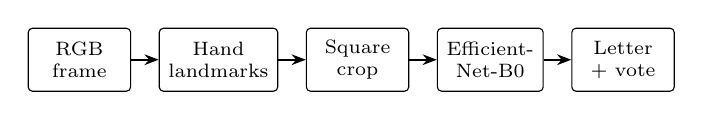
\begin{tikzpicture}[
  node distance=3.5mm,
  box/.style={draw, rounded corners=1.5pt, minimum height=8mm, minimum width=13mm, font=\scriptsize, align=center},
  arr/.style={-{Stealth[length=1.8mm]}, thick}]
\node[box] (a) {RGB\\frame};
\node[box, right=of a] (b) {Hand\\landmarks};
\node[box, right=of b] (c) {Square\\crop};
\node[box, right=of c] (d) {Efficient-\\Net-B0};
\node[box, right=of d] (e) {Letter\\+ vote};
\draw[arr] (a)--(b); \draw[arr] (b)--(c); \draw[arr] (c)--(d); \draw[arr] (d)--(e);
\end{tikzpicture}
\caption{Recognition pipeline. MediaPipe localizes the hand, a square crop is classified by EfficientNet-B0, and a short temporal vote stabilizes the live output.}
\label{fig:pipeline}
\end{figure}

\subsection{Classifier}
We use EfficientNet-B0~\cite{tan2019efficientnet} initialized from ImageNet~\cite{deng2009imagenet} weights. The original 1000-way classification layer is replaced by a new 26-way linear layer, and all layers are fine-tuned. The final model has 4.04\,M parameters. The network is trained with the cross-entropy loss
\begin{equation}
\mathcal{L} = -\frac{1}{B}\sum_{i=1}^{B}\log \frac{\exp(z_{i,y_i})}{\sum_{k=1}^{26}\exp(z_{i,k})},
\end{equation}
where $z_{i,k}$ is the logit of class $k$ for sample $i$, $y_i$ its label and $B$ the batch size.

\subsection{Training Configurations}
We train three models that differ only in the input and augmentation policy.

\textbf{Full image (F).} The original, uncropped image is used.

\textbf{Hand crop (C).} Each training image is replaced by its cached hand crop. Standard augmentation is applied: random resized crop (scale 0.8--1.0), horizontal flip with probability 0.3, rotation up to $15^\circ$ and color jitter (brightness and contrast 0.3, saturation 0.2, hue 0.1)~\cite{shorten2019survey}.

\textbf{Hand crop with robust augmentation (C+R).} Same crops, but the augmentation is designed against the failure modes we expect in deployment: the flip probability is raised to 0.5 because signers use either hand, brightness and contrast jitter is increased to 0.5 and saturation to 0.3, random grayscale (probability 0.1) and Gaussian blur (probability 0.2, $\sigma\in[0.1,2.0]$) imitate low-quality webcams, and the random-crop scale is widened to 0.6--1.0 to tolerate imperfect crops.

\subsection{Optimization}
All models use AdamW~\cite{loshchilov2019decoupled} with learning rate $2\times10^{-4}$, weight decay $10^{-4}$, batch size 16 and 5 epochs. The learning rate follows a cosine schedule~\cite{loshchilov2017sgdr} with a linear warm-up over the first 5\% of steps. Training uses automatic mixed precision. At the end of each epoch the model is evaluated on the validation split, and the checkpoint with the highest validation accuracy is retained for testing.

\section{Experimental Setup}
\label{sec:setup}
\subsection{Metrics}
We report top-1 accuracy, macro-averaged F1 score, per-class precision and recall, and the normalized confusion matrix on the test split. We also report the parameter count and two timings, both measured on a laptop with an NVIDIA GeForce RTX 3050 Laptop GPU and a 12-thread CPU: (i) \emph{model-inference latency}, the time of one forward pass of the network on a single pre-processed $224\times224$ image (batch size 1, mean of 100 repetitions after 10 warm-up passes, excluding image loading, hand detection and cropping), and (ii) \emph{end-to-end throughput} of the full live pipeline (hand detection, cropping, pre-processing and classification), in frames per second.

\subsection{Implementation}
Models are implemented in PyTorch with pretrained weights loaded through the \texttt{transformers} library, and hand localization uses the MediaPipe Tasks API. All experiments use a single run with seed 42; we did not average over seeds, so differences of a few images between models are not statistically meaningful (Section~\ref{sec:discussion}).

\section{Results}
\label{sec:results}

\subsection{In-Distribution Performance}
Table~\ref{tab:main} summarizes the results. All three configurations exceed 98.9\% test accuracy. The full-image model attains the highest test accuracy (99.45\%, 6 errors in 1{,}088 images), the robust crop model follows (99.36\%, 7 errors) and the standard crop model is lowest (98.90\%, 12 errors). The macro-F1 scores track accuracy closely, which is expected because the test split is almost perfectly balanced across classes. A 95\% binomial confidence interval around 99.4\% with $n=1{,}088$ is roughly $\pm0.5$ points, so the three models are not clearly separable on this split alone.

\begin{table}[t]
\caption{Results for the three configurations on the 1{,}088-image held-out test split. Latency is model-inference latency only (one forward pass, batch size 1, RTX 3050 Laptop GPU), not end-to-end pipeline latency.}
\label{tab:main}
\centering
\small
\begin{tabular}{@{}lcccc@{}}
\toprule
\textbf{Model} & \textbf{Test acc.} & \textbf{Macro-F1} & \textbf{Params} & \textbf{Latency}\\
 & (\%) & & (M) & (ms)\\
\midrule
Hand crop (C) & 98.90 & 0.989 & 4.04 & 12.4\\
Hand crop + robust (C+R) & 99.36 & 0.994 & 4.04 & 13.9\\
Full image (F) & \textbf{99.45} & \textbf{0.995} & 4.04 & 13.1\\
\bottomrule
\end{tabular}
\end{table}

Fig.~\ref{fig:curves} shows the learning curves of the robust crop model. Training and validation losses fall together, and validation accuracy reaches 99.36\% at epoch 4; the slight decline at epoch 5 (98.16\%) is within the epoch-to-epoch noise of a 1{,}087-image validation split, and the epoch-4 checkpoint is the one evaluated on the test set. We observed the same pattern for the standard crop model (best at epoch 4), whereas the full-image model peaked at epoch 5.

\begin{figure}[t]
\centering
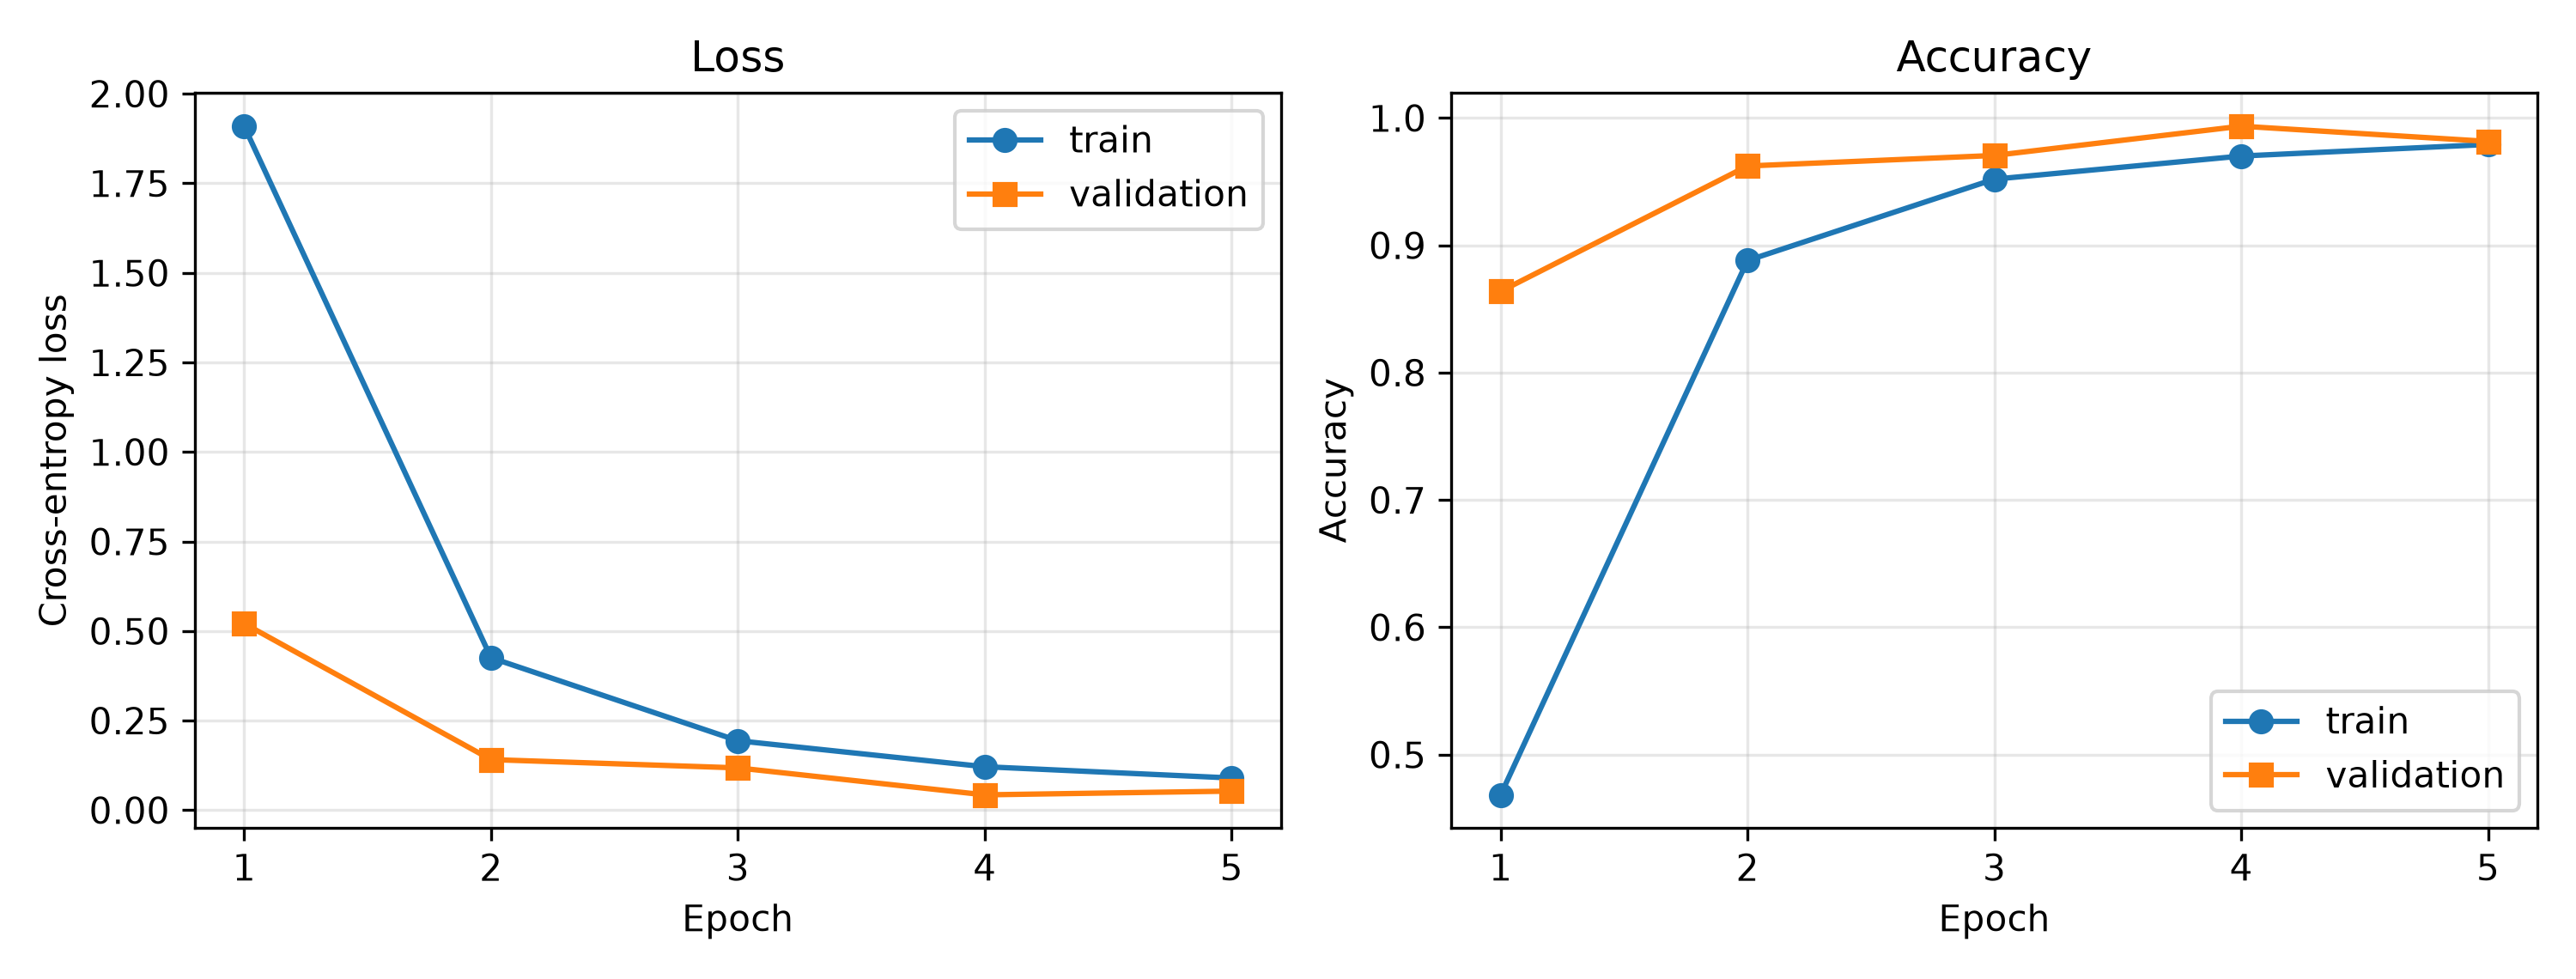
\includegraphics[width=\columnwidth]{fig_curves.png}
\caption{Training and validation loss (left) and accuracy (right) of the robust crop model over five epochs.}
\label{fig:curves}
\end{figure}

\subsection{Per-Class Analysis}
For the robust crop model, 16 of 26 classes reach an F1 score of 1.000 on the test split. The lowest F1 scores are for Z (0.964; recall 0.952), R (0.976) and J (0.977). The normalized confusion matrix is shown in Fig.~\ref{fig:confusion}. The few errors involve handshapes that are close in appearance. For the standard crop model, the weakest class was F (recall 0.905), confused mainly with B, followed by M and R (recall 0.952 each); N and S received many of the misassigned predictions. M, N and S are closed-fist letters distinguished by thumb position and the number of folded fingers. Z and J are the two letters that depend on motion in real signing; a static image can only capture one pose along the trajectory, which makes them intrinsically harder.

\begin{figure}[t]
\centering
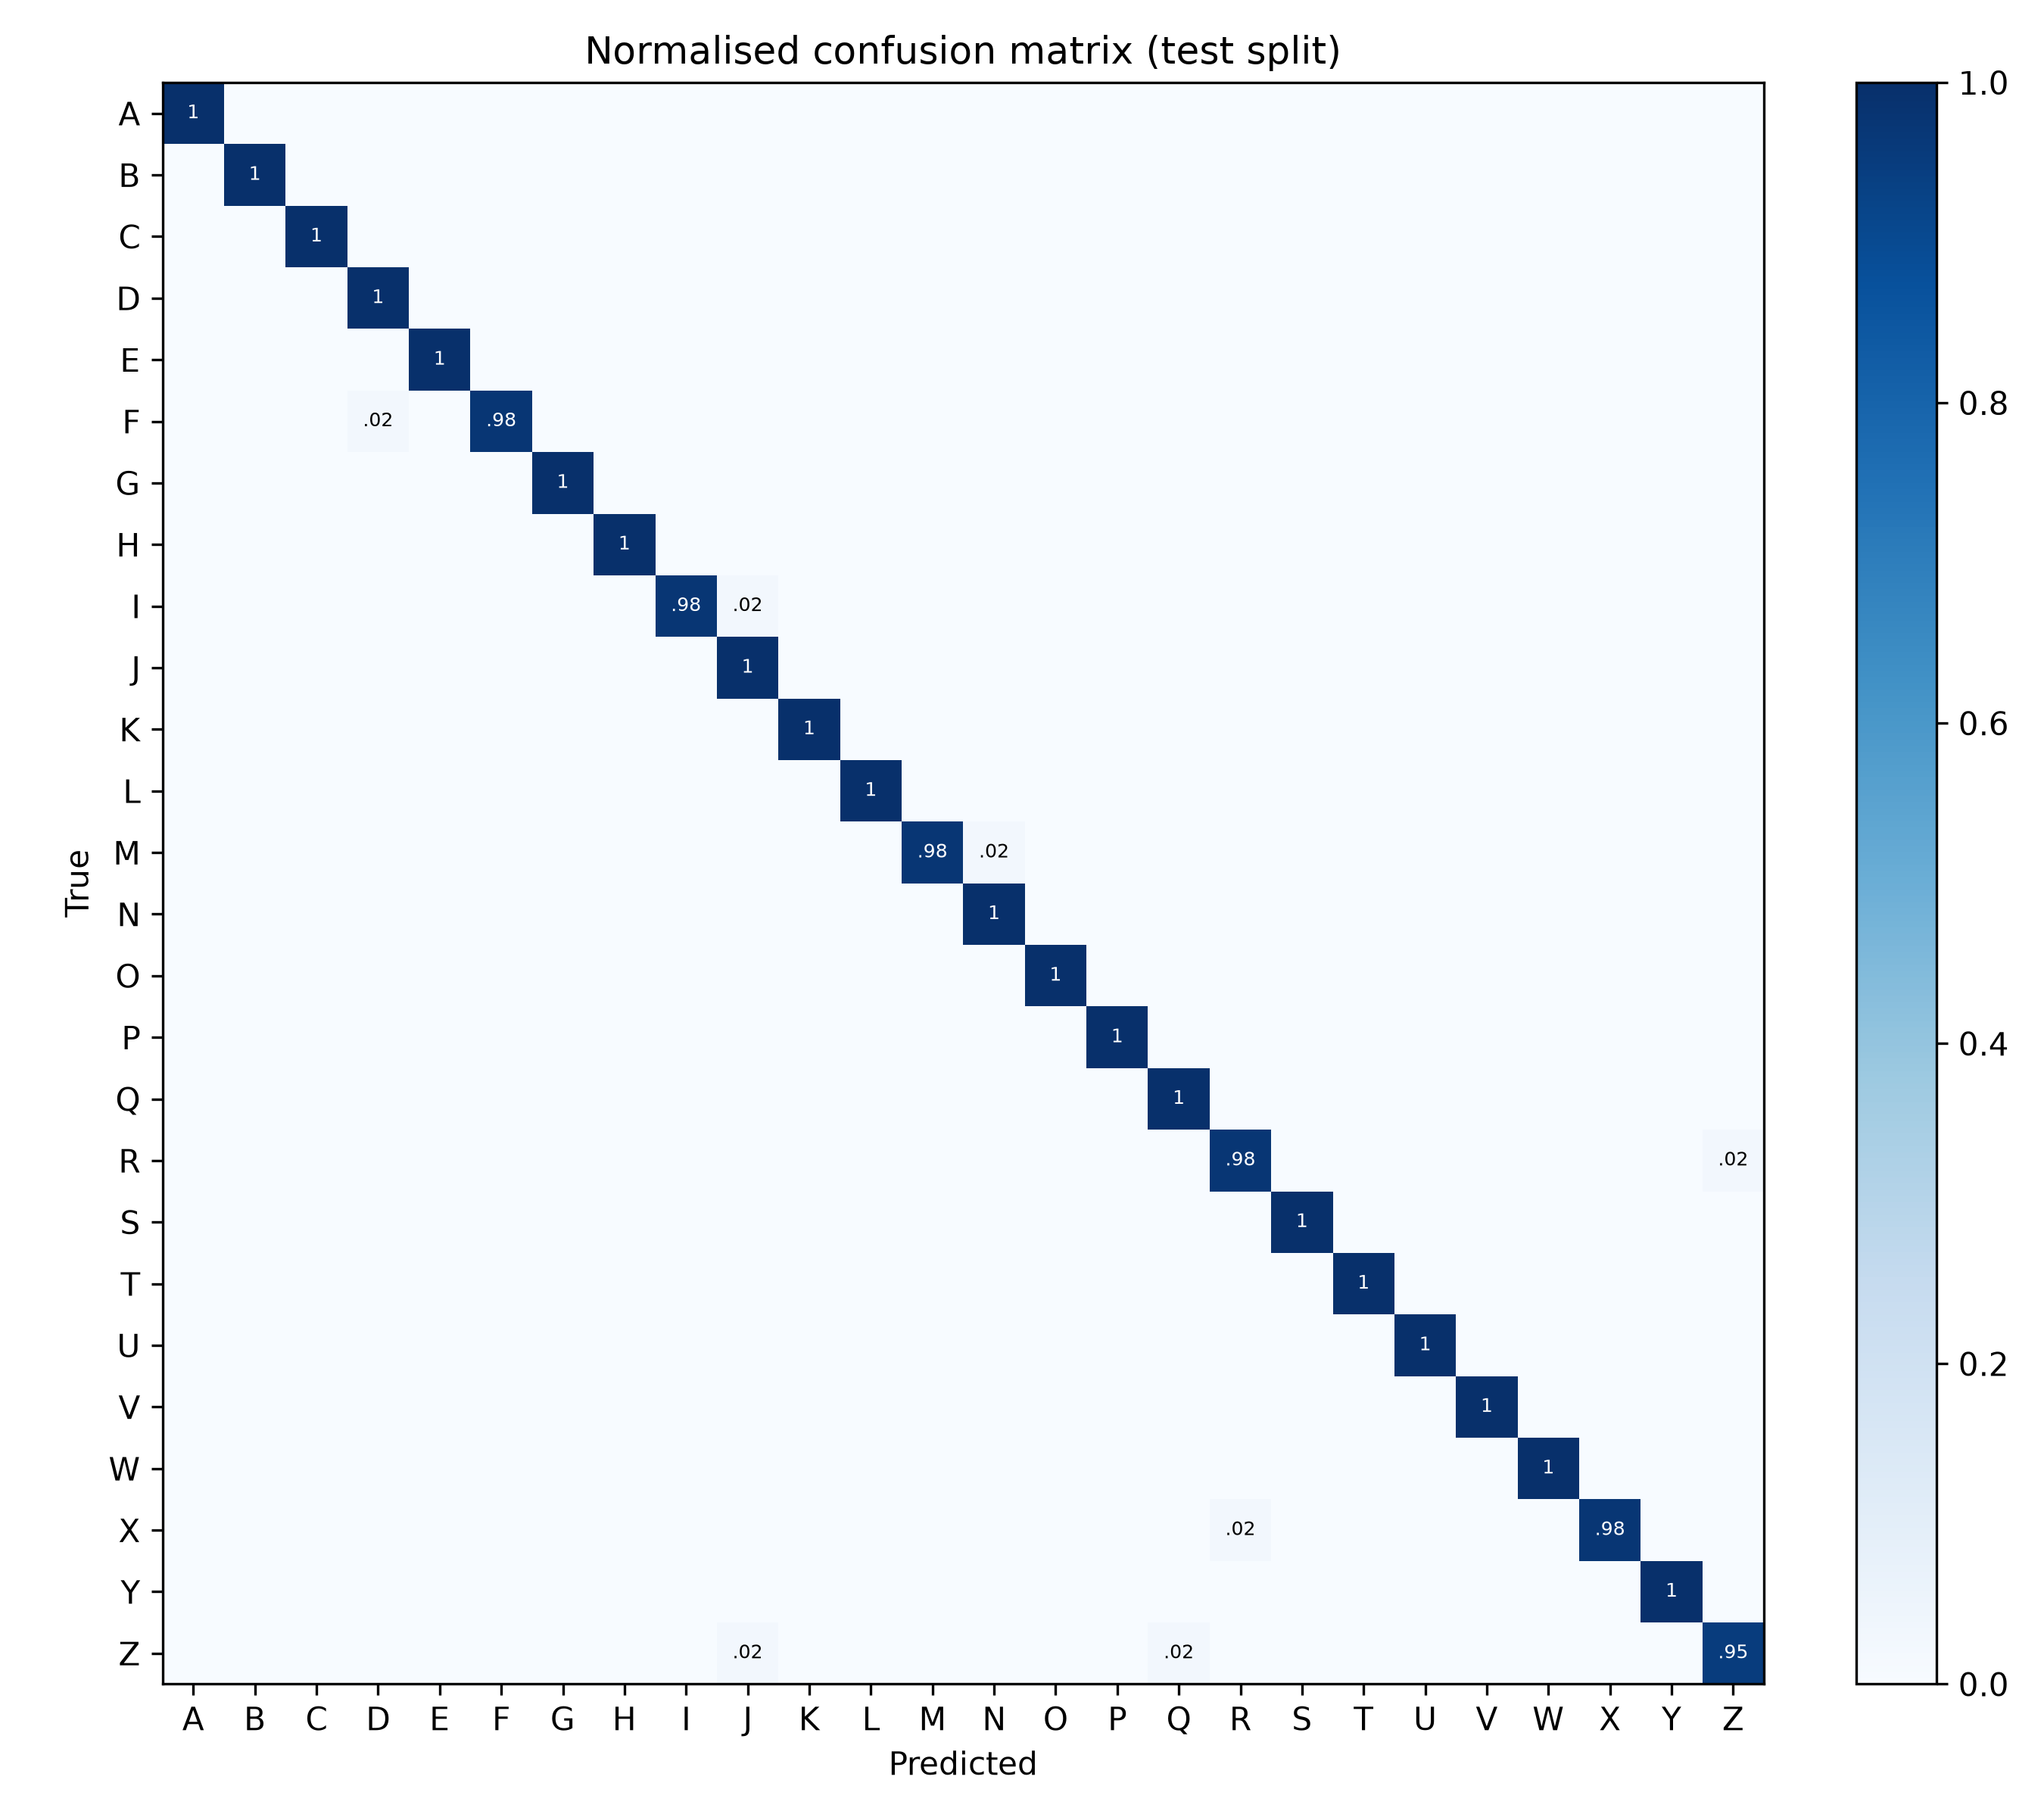
\includegraphics[width=0.98\columnwidth]{fig_confusion.png}
\caption{Normalized confusion matrix of the robust crop model on the 1{,}088-image test split. Off-diagonal mass is small and limited to visually similar letters.}
\label{fig:confusion}
\end{figure}

\subsection{Efficiency}
Each model has 4.04\,M parameters. Model-inference latency (forward pass only, batch size 1) on the RTX 3050 Laptop GPU is 12.4\,ms (C), 13.9\,ms (C+R) and 13.1\,ms (F); the differences reflect measurement noise, since the architectures are identical. Hand localization is not included in these figures. End to end, the crop pipeline (MediaPipe hand detection in video mode, cropping, pre-processing and classification) ran at 18.2 frames per second in an offline benchmark of 208 frames of size $640\times480$ replayed from still images (hand found in 168 of them; hand detection 24.9\,ms per frame on average). This benchmark excludes camera capture and display, so the frame rate of a live session may be somewhat lower; it is nevertheless sufficient for live fingerspelling.

\subsection{Comparison of Configurations}
The three configurations differ by only 1 to 6 test images: 12 errors for C, 7 for C+R and 6 for F. A 95\% binomial interval around 99.4\% with $n=1{,}088$ is roughly $\pm0.5$ points and all results come from a single seed, so the ordering of the models is not statistically reliable. We conclude only that all three configurations reach comparable in-distribution accuracy. In particular, hand cropping did not improve held-out accuracy over using the full frame. The robust augmentation policy reduced errors from 12 to 7 relative to the standard crop policy on this split, a difference of five images.

\section{Discussion}
\label{sec:discussion}
\textbf{Does cropping help?} In our experiments cropping did not improve the in-distribution result: the full-image model was marginally best on the test split. On the dataset's own images the full frame carries additional context, including consistent backgrounds within some classes, which a network can exploit, so this split cannot reveal whether the crop pipeline is more robust to background changes. The crop pipeline remains attractive because it provides an explicit, interpretable region of interest and is intended for live use in cluttered scenes, but demonstrating that benefit requires evaluation on independent data.

\textbf{Scope of the evaluation.} All reported accuracies are measured on a random held-out split of a single dataset. They describe how well the models learned this dataset's distribution, and they should not be read as the accuracy to expect for new signers, cameras or lighting conditions, because images from one dataset share signers, cameras and backgrounds\~\cite{torralba2011unbiased,quinonero2009dataset}. We did not evaluate cross-signer generalization.

\textbf{Limitations.} (1) The evaluation is in-distribution only. (2) Results come from a single seed and a single split, and differences of a few images between models are not meaningful. (3) J and Z cannot be fully represented by a single frame; a temporal model would be needed for them, and some fingerspelling studies evaluate the 24 static letters separately. (4) The dataset has limited signer diversity, and we did not evaluate across skin tones, hand sizes or camera types. (5) Only isolated letters are recognized; continuous fingerspelling and word-level recognition are not addressed. (6) We did not compare against other architectures under the same protocol, so our conclusions concern EfficientNet-B0 specifically.

\textbf{Future work.} Priorities are (a) a multi-signer benchmark collected before any model selection, (b) leave-signer-out cross-validation, (c) temporal models for J and Z, (d) landmark-based features combined with appearance, which are less sensitive to background and lighting, and (e) comparison with other efficient backbones\~\cite{sandler2018mobilenetv2,dosovitskiy2021image}.

\section{Conclusion}
\label{sec:conclusion}
We presented a real-time ASL alphabet recognizer built from MediaPipe hand localization and a fine-tuned EfficientNet-B0 with only 4.04\,M parameters. All three configurations reached 98.9--99.5\% accuracy on a held-out split of 1{,}088 images and run in about 13\,ms per image on a laptop GPU. The remaining errors are concentrated in visually similar handshapes and in the motion-based letters J and Z. Because the evaluation is in-distribution, these figures do not establish performance on unseen signers or capture conditions, which we identify as the main direction for future work.

\begin{thebibliography}{00}
\bibitem{rastgoo2021survey} R. Rastgoo, K. Kiani, and S. Escalera, ``Sign language recognition: A deep survey,'' \emph{Expert Systems with Applications}, vol. 164, Art. no. 113794, 2021.
\bibitem{cheok2019review} M. J. Cheok, Z. Omar, and M. H. Jaward, ``A review of hand gesture and sign language recognition techniques,'' \emph{Int. J. Machine Learning and Cybernetics}, vol. 10, pp. 131--153, 2019.
\bibitem{koller2020quantitative} O. Koller, ``Quantitative survey of the state of the art in sign language recognition,'' arXiv:2008.09918, 2020.
\bibitem{shi2018fingerspelling} B. Shi, A. Martinez Del Rio, J. Keane, J. Michaux, D. Brentari, G. Shakhnarovich, and K. Livescu, ``American Sign Language fingerspelling recognition in the wild,'' in \emph{Proc. IEEE Spoken Language Technology Workshop (SLT)}, 2018, pp. 145--152.
\bibitem{pugeault2011spelling} N. Pugeault and R. Bowden, ``Spelling it out: Real-time ASL fingerspelling recognition,'' in \emph{Proc. IEEE Int. Conf. Computer Vision Workshops (ICCV Workshops)}, 2011, pp. 1114--1119.
\bibitem{kang2015realtime} B. Kang, S. Tripathi, and T. Q. Nguyen, ``Real-time sign language fingerspelling recognition using convolutional neural networks from depth map,'' in \emph{Proc. 3rd IAPR Asian Conf. Pattern Recognition (ACPR)}, 2015, pp. 136--140.
\bibitem{pigou2014sign} L. Pigou, S. Dieleman, P.-J. Kindermans, and B. Schrauwen, ``Sign language recognition using convolutional neural networks,'' in \emph{Proc. ECCV Workshops}, LNCS vol. 8925, 2014, pp. 572--578.
\bibitem{li2020word} D. Li, C. Rodriguez, X. Yu, and H. Li, ``Word-level deep sign language recognition from video: A new large-scale dataset and methods comparison,'' in \emph{Proc. IEEE Winter Conf. Applications of Computer Vision (WACV)}, 2020, pp. 1459--1469.
\bibitem{tan2019efficientnet} M. Tan and Q. V. Le, ``EfficientNet: Rethinking model scaling for convolutional neural networks,'' in \emph{Proc. Int. Conf. Machine Learning (ICML)}, PMLR vol. 97, 2019, pp. 6105--6114.
\bibitem{deng2009imagenet} J. Deng, W. Dong, R. Socher, L.-J. Li, K. Li, and L. Fei-Fei, ``ImageNet: A large-scale hierarchical image database,'' in \emph{Proc. IEEE Conf. Computer Vision and Pattern Recognition (CVPR)}, 2009, pp. 248--255.
\bibitem{krizhevsky2012imagenet} A. Krizhevsky, I. Sutskever, and G. E. Hinton, ``ImageNet classification with deep convolutional neural networks,'' in \emph{Advances in Neural Information Processing Systems (NIPS)}, vol. 25, 2012, pp. 1097--1105.
\bibitem{simonyan2015very} K. Simonyan and A. Zisserman, ``Very deep convolutional networks for large-scale image recognition,'' in \emph{Proc. Int. Conf. Learning Representations (ICLR)}, 2015.
\bibitem{he2016deep} K. He, X. Zhang, S. Ren, and J. Sun, ``Deep residual learning for image recognition,'' in \emph{Proc. IEEE Conf. Computer Vision and Pattern Recognition (CVPR)}, 2016, pp. 770--778.
\bibitem{howard2017mobilenets} A. G. Howard \emph{et al.}, ``MobileNets: Efficient convolutional neural networks for mobile vision applications,'' arXiv:1704.04861, 2017.
\bibitem{sandler2018mobilenetv2} M. Sandler, A. Howard, M. Zhu, A. Zhmoginov, and L.-C. Chen, ``MobileNetV2: Inverted residuals and linear bottlenecks,'' in \emph{Proc. IEEE Conf. Computer Vision and Pattern Recognition (CVPR)}, 2018, pp. 4510--4520.
\bibitem{dosovitskiy2021image} A. Dosovitskiy \emph{et al.}, ``An image is worth 16x16 words: Transformers for image recognition at scale,'' in \emph{Proc. Int. Conf. Learning Representations (ICLR)}, 2021.
\bibitem{yosinski2014transferable} J. Yosinski, J. Clune, Y. Bengio, and H. Lipson, ``How transferable are features in deep neural networks?'' in \emph{Advances in Neural Information Processing Systems (NIPS)}, vol. 27, 2014, pp. 3320--3328.
\bibitem{pan2010survey} S. J. Pan and Q. Yang, ``A survey on transfer learning,'' \emph{IEEE Trans. Knowledge and Data Engineering}, vol. 22, no. 10, pp. 1345--1359, Oct. 2010.
\bibitem{zhang2020mediapipe} F. Zhang \emph{et al.}, ``MediaPipe Hands: On-device real-time hand tracking,'' arXiv:2006.10214, 2020.
\bibitem{lugaresi2019mediapipe} C. Lugaresi \emph{et al.}, ``MediaPipe: A framework for building perception pipelines,'' arXiv:1906.08172, 2019.
\bibitem{shorten2019survey} C. Shorten and T. M. Khoshgoftaar, ``A survey on image data augmentation for deep learning,'' \emph{J. Big Data}, vol. 6, Art. no. 60, 2019.
\bibitem{loshchilov2019decoupled} I. Loshchilov and F. Hutter, ``Decoupled weight decay regularization,'' in \emph{Proc. Int. Conf. Learning Representations (ICLR)}, 2019.
\bibitem{loshchilov2017sgdr} I. Loshchilov and F. Hutter, ``SGDR: Stochastic gradient descent with warm restarts,'' in \emph{Proc. Int. Conf. Learning Representations (ICLR)}, 2017.
\bibitem{quinonero2009dataset} J. Qui{\~n}onero-Candela, M. Sugiyama, A. Schwaighofer, and N. D. Lawrence, Eds., \emph{Dataset Shift in Machine Learning}. Cambridge, MA, USA: MIT Press, 2009.
\bibitem{bendavid2010theory} S. Ben-David, J. Blitzer, K. Crammer, A. Kulesza, F. Pereira, and J. W. Vaughan, ``A theory of learning from different domains,'' \emph{Machine Learning}, vol. 79, pp. 151--175, 2010.
\bibitem{torralba2011unbiased} A. Torralba and A. A. Efros, ``Unbiased look at dataset bias,'' in \emph{Proc. IEEE Conf. Computer Vision and Pattern Recognition (CVPR)}, 2011, pp. 1521--1528.
\end{thebibliography}

\end{document}
